


\chapter{Acoustic feature extraction and classification techniques used for Spoken language recognition}
%\chaptermark{Acoustic feature extraction and classification techniques used for Spoken language recognition}
\HRule \\[-0.5cm] % Horizontal line

%\label{Chapter2} % For referencing the chapter elsewhere, use \ref{Chapter1}

%\lhead{\emph{\textbf{Chapter2:} Acoustic feature extraction and classification techniques used for Spoken language recognition}} % This is for the header on each page - perhaps a shortened title

%----------------------------------------------------------------------------------------
%	SECTIONS
%----------------------------------------------------------------------------------------
\begin{spacing}{1.5}
The acoustic information is generally considered as the first level analysis of speech production. Human speech is a longitudinal pressure wave, and different speech events can be distinguished at an acoustic level, according to amplitude and frequency components of the waves. The acoustic information is one of the simplest forms of information, which can be obtained during the speech parameterization process directly from raw speech. The higher level of speech information like phonotactic and word information can also be extracted from the acoustic information~\cite{ambikairajah2011language}. For the spoken language recognition task, the Mel frequency cepstral coefficients (MFCC) are the most widely used feature extraction technique. The language discriminative information largely reflects on the temporal patterns of the speech signal. Thus, once the basic acoustic features have been obtained, additional features are appended to each feature vectors. Some commonly utilized additional features are the delta and acceleration cepstrum (MFCC + delta + acceleration) and the shifted delta cepstrum (SDC).

\section{Mel frequency cepstral coefficients (MFCC)}
The Mel frequency cepstral coefficients (MFCCs) are one of the most commonly used filter-bank based parameterization method for speech processing applications, such as speech recognition, speaker verification/identification and spoken language recognition. The human perception of the frequency content of the sound follows a nonlinear scale called Mel scale~\cite{chakroborty2009improved}. So, the Mel-scale is used to approximate the nonlinear frequency resolution of the human ear. After the magnitude-square of the Fourier Transform is calculated for the input windowed frame of speech, it is passed through a bank of triangular Mel filters and the natural logarithm of the filter bank energies is taken. As the filter bank log-energies are highly correlated, a linear transformation technique (I.e the Discrete Cosine Transform (DCT)) is used to de-correlate the information yielding in Mel frequency cepstral coefficients. The steps to extract MFCC Features from speech sample is depicted in figure~\ref{mfcc}. The brief description of all the steps are as follows.
\begin{figure}[h]
\centering{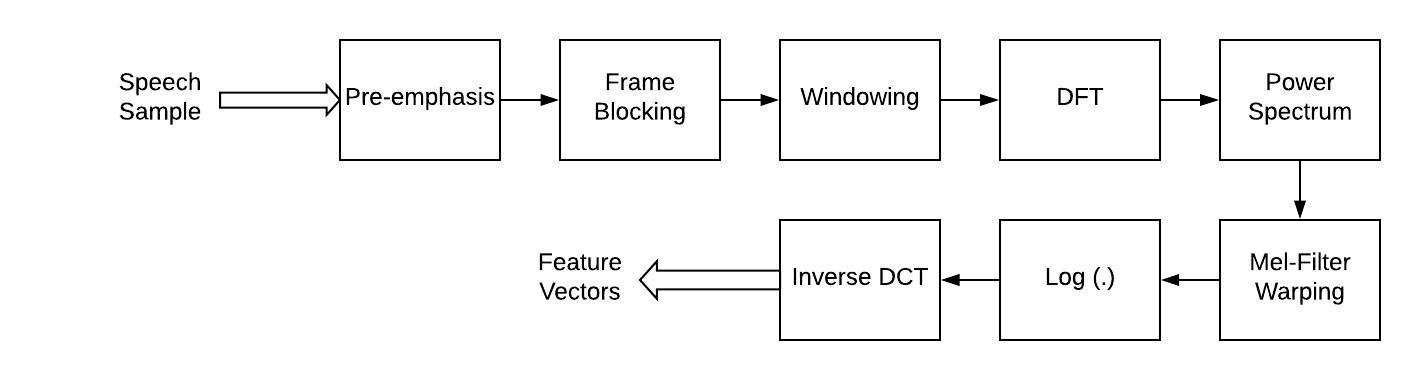
\includegraphics[scale=.55]{Images/mfcc.jpeg}}
\caption{Block diagram of MFCC extraction.}
\label{mfcc}
\end{figure} 
\subsection{Pre-emphasis}
\begin{figure}[h]
\centering{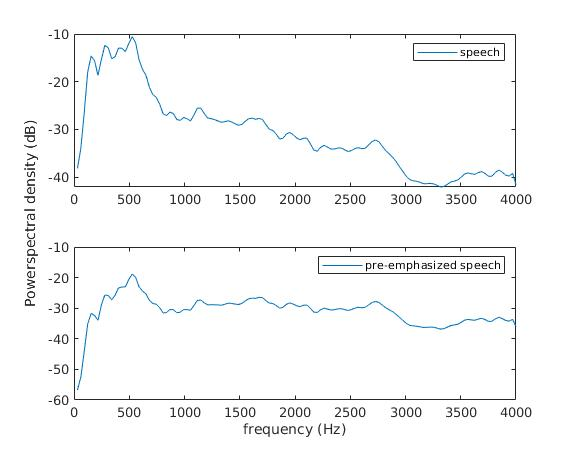
\includegraphics[scale=.55]{Images/pre_effect.jpg}}
\caption{The power spectral density of the original speech signal and pre-emphasized speech signal sampled at 8000 Hz.}
\label{pemp}
\end{figure} 
Figure~\ref{pemp} shows the power spectral density of the original speech and its pre-emphasized speech. It has been observed from the figure that the power of the signal falls sharply in high frequency regions. It is estimated that about 80\% of the power is contained within frequency components below 1000 Hz~\cite{beigi2011speaker}. To perform verious recognition task human ear's cochlea utilizes a fine-tuning mechanism based on feedback from the brain that amplifies special frequencies. Therefore the human ear can easily recognize these low energy regions. Since our objective is to design a recognition system, we have to do something to enhance the high frequency components, by which high frequency information can also play a role in recognition task. This can be achieved through pre-emphasis. One method which has been used quite often is a differentiator (single zero filter), whose transfer function is given in equation~\ref{pr}  


\begin{equation}
\label{pr}
    H_{p}(z)=1-\alpha z^{-1}
\end{equation}
The most popular range of values for $ \alpha $ is between 0.95 and 0.97, although values in the range of 0.9 and just less than 1.0 have also been used in different systems.
Figure~\ref{pemp} shows the power spectral density of the pre-emphasized signal using $ \alpha=0.98 $. Here we notice that the absolute power for each frequency range has been reduced, but the relative power is better distributed along the different frequencies.

\subsection{Frame blocking} The speech is slow varying quasi-stationary signal.
Therefore, speech analysis must always be carried out on short segments across which the speech signal is assumed to be stationary. Short-term spectral measurements are typically carried out over the range of 10-30 ms frame size and shift~\cite{beigi2011speaker}. In that direction, the speech signal is divided into frames of L samples, with adjacent frames being separated by M samples with the value M less than that of L. The first frame consists of the first L samples. The second frame begins from M samples after the first frame, and overlaps it by L - M samples and so on. This process continues until all the speech samples are taken into account.

\subsection{Windowing} The next step is to window each individual frame to minimize the signal discontinuities at the beginning and end of each frame. The concept applied here is to minimize the spectral distortion by using the window to taper the signal to zero at the beginning and end of each frame. If we define the window as w(n), $0 \leq n \leq L-1$  where L is the frame length, then the result of windowed signal can be written as:
\begin{equation}
 s_{o}(n)=w(n).s_{i}(n)
\end{equation} 
where w(n) the window function. In general hamming window (to eliminate the problem of spectral leakage and zero offset) is widely used to analyze the speech frames.


\begin{equation}
 w(n)=0.54-0.46cos\Bigg(\frac{2\pi n}{L-1}\Bigg), 0\leq n \leq L-1
\end{equation} 


\subsection{DFT} The next step in the processing of the speech data to be able to compute its spectral features is to take a Discrete Fourier Transform of the windowed data. The DFT is computed using equation~\ref{dft}. The DFT length L is always grater then the windowed speech segments length to avoid time aliasing.

\begin{equation}
 \label{dft}
 S(k)=\sum_{n=0}^{L-1}s(n).e^{\frac{-j2\pi kn}{L}}, 1 \leq k \leq L-1, 1 \leq n \leq L-1
\end{equation}


\subsection{Power spectrum}  The loudness is related with intensity of the signal, hence our goal is to convert it into a value that would represent loudness so that we may mimic human perception. Therefore, after the calculation of DFT of each windowed speech segment the power spectrum ($|{S(K)}|^2$) is calculated.


\subsection{Mel filter warping} The human auditory perception is based on a scale which is somewhat linear up to the frequency of 1000 Hz and then becomes close to logarithmic for the higher frequencies.  This was the motivation to use the Mel scale. It has been seen from the literature, that the 24 band filter bank is used to model the auditory system~\cite{beigi2011speaker}. The designed 24 Mel filter banks are presented in figure~\ref{Mel}. First the lowest and highest frequency is converted to Mel scale using equation~\ref{hz2mel}. The unity height triangular filters are uniformly spaced in Mel scale, so in Mel scale the difference between the lowest and highest frequency are uniformly divided into M (no of filter)+1 segments to find the center frequency of each filter. Then the center frequencies which are in Mel scale are converted to Hz scale using equation~\ref{Mel2hz}~\cite{chakroborty2009improved}. The triangular filter banks ($H_{m}(k)$) can be constructed using equation~\ref{trf}. $\{k_{c_{m}}\}_{m=1}^{M}$ are the center frequencies of the filter, $k_{c_{0}}$ and $k_{c_{M+1}}$  are the boundary frequencies in Hz scale (lowest and highest frequency). The output of the Mel filter bank can be computed using equation~\ref{sMel}. Where $H_{m}(k)$ is the filter bank function and M is the no of filter bank used.

\begin{figure}[ht]
\centering{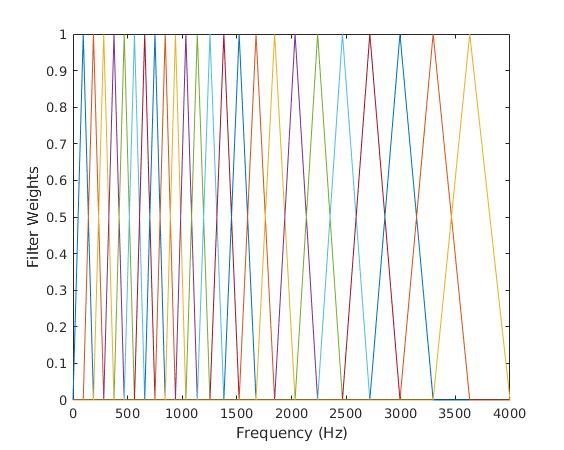
\includegraphics[scale=.35]{Images/mel.jpg}}
\caption{Shape of Mel filter bank for a 24 filter system with sampling frequency of 8000 Hz .}
\label{Mel}
\end{figure} 

\begin{equation}
f_{Mel}=2595 ~.~ log_{10}\Big(1+\frac{f_{lin}}{700}\Big)
%f=f_{high}+f_{low}-f_{Mel2hz}[f_{Mel}(f_{high})+f_{Mel}(f_{low})-f_{Mel}(f)]
\label{hz2mel}
\end{equation}

\begin{equation}
f_{lin}=700.\Big(10^{\frac{f_{mel}}{2595}}-1\Big)
%f=f_{high}+f_{low}-f_{Mel2hz}[f_{Mel}(f_{high})+f_{Mel}(f_{low})-f_{Mel}(f)]
\label{Mel2hz}
\end{equation}

\begin{equation}
H_{m}(k) =
\begin{cases}
0 & \text{for $k \leq k_{c_{m-1}}$}\\
\frac{k-k_{c_{m-1}}}{k_{c_{m}}-k_{c_{m-1}}} & \text{for $k_{c_{m-1}} \leq k \leq k_{c_{m}}$} \\
\frac{k_{c_{m+1}}-k}{k_{c_{m+1}}-k_{c_{m}}} & \text{for $k_{c_{m}} \leq k \leq k_{c_{m+1}}$} \\
0 & \text{for $k \geq k_{c_{m+1}}$}, \quad 1 \leq m \leq M
\end{cases}
\label{trf}
\end{equation}

\begin{equation}
 \label{sMel}
 S(m)=\sum_{k=1}^{N}|S(k)|^{2}H_{m+1}(k), 0 \leq m \leq M-1
\end{equation}



\subsection{log(.)} 
Now we have to warp the power spectra into a logarithmic scale. As we know the dynamic range of the power spectra very high in between different Mel frequency bands, so logarithm with base 10 is used to reduce the dynamic range. It has been seen that in human perception, the vocal tract response information plays a vital role to recognize speaker and language. In time domain the vocal tract response and excitation response are convoluted, therefore in frequency domain they are multiplied. The use of log(.), converts multiplication to addition, latter low time liftering is used to enhance the vocal tract information.    
\subsection{Inverse DCT}
In the previous section we computed the log of the power spectral density of the signal in Mel scale. By taking inverse discrete cosine transform (DCT), we will get the cepstrum of the signal. The most attractive features of the cepstrum is its inherent invariance toward linear spectral distortions, which make it a good candidate for usage in speaker and language recognition task. We can also compute the cepstrum using inverse discrete Fourier transform, but in that case the coefficients are complex (s(m) is not symmetric). One possibility is to take square magnitude of the coefficients or to use inverse DCT directly to get real coefficients. The coefficients using inverse DCT is computed using equation~\ref{dct}.     

\begin{equation}
 \label{dct}
 c(n)=\sum_{m=0}^{M-1}a_{m}log_{10}(S(m))cos\Bigg(\frac{\pi n(m-0.5)}{M}\Bigg), 0 \leq n \leq C-1
\end{equation}


    $$ a_{m}=
   \begin{cases}
    \frac{1}{M} & \text{for $m=0$} \\
     \frac{2}{M} & \text{for $m > 0$}
   \end{cases}$$

Where C is the no of cepstral coefficients needs to be computed and DCT length M should be always grater then or equal to the no of filter bank used to compute Mel coefficients.

\section{Delta and Delta-Delta cepstra ($\Delta$ and $\Delta-\Delta$)}

The static MFCC feature vectors provides a good estimation of local spectra, but it fails to capture the dynamics of human speech. The dynamics of human speech is very important information for distinguishing different     languages~\cite{ambikairajah2011language}.  Therefore, the performance of the system greatly enhanced by adding time derivative of basic static parameters. The Delta and Delta-Delta provides an estimation of local temporal derivatives of the speech cepstrum, and are implemented as a least square approximation of the local slope and calculated over multiple frames. The first order derivative are computed as delta coefficients and can be computed as per equation~\ref{del}.

\begin{equation}
\label{del}
    \Delta c_{i}(n)=\frac{\sum _{k=-N}^{k=N}kc_{i}(n+k)}{\sum _{k=-N}^{k=N}k^2}
\end{equation}
Where $\Delta c_{i}(n)$ is the delta coefficient of the $i^{th} $ cepstral stream and $n^{th} $ frame. The N defines the no of frames to be used for the computation of delta coefficients. Typically the range of N is from 2 to 4. Similarly the $\Delta-\Delta$ coefficients are computed using the same equation on Delta coefficients instead of static coefficients. As the Delta and Delta-Delta coefficients computation needs the coefficients of previous and post frame, needs some modification at beginning and end of speech. This end-effect
problem can be solved by using simple first order differences at the start and end of the speech (as per equation ~\ref{start} and ~\ref{end}).
\begin{equation}
\label{start}
    \Delta c_{i}(n)=c_{i}(n+1)-c_{i}(n),\quad n < N
\end{equation}
\vspace{-0.5 cm }
\begin{equation}
\label{end}
    \Delta c_{i}(n)=c_{i}(n)-c_{i}(n-1),\quad n \geq T-N
\end{equation}
Where T is the total no of frames. In general the delta and delta-delta cepstrum are concatenated with the static cepstrum to form a single
feature vector containing both the static and dynamic
information of the speech signal.

\section{Shifted delta coefficients (SDC)}
The delta and delta-delta feature able to capture the temporal information, But it is limited, and not able to capture the higher level temporal dynamics information. If we consider $N=2$, the delta and delta-delta can able to capture the temporal dynamics information across 5 frames, i.e. across 50 ms (if $frameshift=10 ms$).

Temporal information has proven useful in distinguishing languages, i.e accessing the likelihood of one phone following another (phonotactic information). Thus, this intuition leads to design a feature, which can capture the temporal dynamics information in a larger window. One way, we can choose larger N value in the delta calculations to include a much longer window in the calculation. But, this will only produce a much longer average of the slope and the finer details will be lost. The SDC feature is a better alternative to capture spectral dynamics in a longer window~\cite{torres2002approaches}. The SDC feature is obtained by concatenating future and past frames delta cepstra with the current feature vector.

In general, the computation of SDC are specified by four parameters: z, d, p, k. z specifies the number of basic cepstral streams to use in the calculation, i.e. the number of basic cepstral coefficients. Each of z cepstral streams are treated separately and SDC values are computed for each of them prior to concatenation with the original cepstral coefficients. p is the number of frames from one delta calculation to the next and k is the total number of delta values concatenated together to form the SDC. The diagram showing the computation procedure of SDC is shown in figure~\ref{sdc}

\begin{figure}[h]
\centering{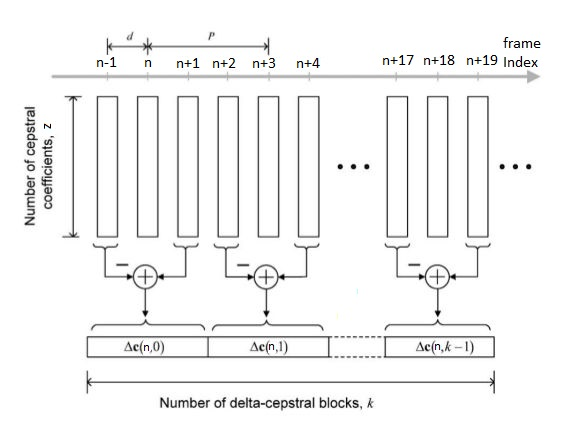
\includegraphics[scale=.55]{Images/sdc.jpg}}
\caption{SDC feature extraction at $n^{th}$ frame, $z-d-p-k=7-1-3-7$.}
\label{sdc}
\end{figure} 
The final parameter d is the difference value used in the delta calculation. for all the SDC calculations the delta values were calculated by subtracting the cepstral value at $n-d$ from that at $n+d$. Thus for each of the M cepstral streams, the final vector at time n is given by the concatenation of all the $\Delta c_{i}(n,z)$ for $0 \leq z \leq k$, where i represents the $i^{th}$ cepstral coefficient. The mathematical equation for the computation of $\Delta c_{i}(n,z)$ is given in equation~\ref{sdc1}.
\begin{equation}
    \label{sdc1}
    \Delta c_{i}(n,z)= c_{i}(n+zp+d)-c_{i}(n+zp-d)
\end{equation}
It has been seen that, the regression based delta computation is more efficient for better estimate then the method of simple subtracting~\cite{ambikairajah2011language}. In this way, the $\Delta c_{i}(n,z)$ can be computed using equation~\ref{sdc2}. 
\begin{equation}
\label{sdc2}
    \Delta c_{i}(n,z)=\frac{\sum _{l=-d}^{l=d}l c_{i}(n+zp+l)}{\sum _{l=-d}^{l=d} l^2}
\end{equation}
With either the standard subtraction method, or the modified regression based technique, the SDC capture temporal dynamics information in a much larger window then the standard delta and delta-delta. In general, people use SDC feature for language recognition task with configuration $z-d-p-k=7-1-3-7$. The best way to compute the SDC feature is, after computing static MFCC (c(n)) and its delta coefficients (d(n)), the SDC coefficients of the $n^{th}$ frame is given as: $$sdc(n)=\Big[c(n), d(n-p),\ldots,d(n),\ldots(d(n+p)) \Big ] $$ 

\section{Gaussian Mixture Model}
\label{gmm_sc}
Gaussian Mixture Model (GMM) is a parametric probability density function represented as a weighted sum of Gaussian component densities. GMMs are capable of representing a large class of sample distributions. Thus, GMMs are commonly used as a parametric model of the probability distribution of continuous measurements or features in a speaker and language recognition systems. 

The use of GMM may also be motivated by the intuitive notion that the individual component densities may model some underlying set of hidden classes. For example, in speaker recognition, it is reasonable to assume the acoustic space of spectral related features corresponding to a speaker’s broad phonetic events, such as vowels, nasals or fricatives. These acoustic classes reflect some general speaker dependent vocal tract configurations that are useful for characterizing speaker identity. The spectral shape of the $i^{th}$ acoustic class can in turn be
represented by the mean $\mu_{i}$ of the $i^{th}$ component density, and variations of the average spectral shape can be represented by the covariance matrix $\Sigma_{i}$. Because all the features used to train the GMM are unlabeled, the acoustic classes are hidden in that the class of an observation is unknown.  GMM parameters are estimated from training data using the iterative expectation-maximization (EM) algorithm or maximum a posteriori (MAP) estimation from a well-trained prior model.

For a D-dimensional feature vector denoted as $X$, the mixture density for a language $S$ is defined as weighted sum of $M_{g}$ component Gaussian densities as given by the following equation~\ref{pr}~\cite{reynolds1995speaker}.
\begin{equation}
\label{pr}
 P(X|S)=\sum_{i=1}^{M_{g}}w_{i}P(X|\theta_{i})
\end{equation} 
where $w_{i}$ are the weights and $P(X|\theta_{i})$ are the component densities. Each component density is a D-variate Gaussian function of parameters $\theta_{i}$ ( $\theta_{i} = \bigg[\mu_{i} \quad  \Sigma_{i}\bigg]$). The probability density function of $P(X|\theta_{i})$ can be written as per equation~\ref{nor} 
\begin{equation}
\label{nor}
 P(X|\theta_{i})=\frac{1}{(2 \pi)^{D/2} |\Sigma_{i}|^{\frac{1}{2}}} \quad e^{-\frac{1}{2}\bigg[(X-\mu_{i})^{T}\Sigma_{i}^{-1}(X-\mu_{i})\bigg]}
\end{equation} 

where $\mu_{i}$ is a mean vector and $\Sigma_{i}$ covariance matrix for $i^{th}$ component. The mixture weights have to satisfy the constraint~\ref{con}~\cite{reynolds1995speaker}.
\begin{equation}
\label{con}
 \sum_{i=1}^{M_{g}}w_{i}=1
\end{equation}
 
 The complete Gaussian mixture density is parameterized by the mean vectors ($\mu_{i}$), the covariance matrices ($\Sigma{i}$) and the mixture weights ($w_{i}$) from all component densities. These parameters are collectively represented by
\begin{equation}
\label{gus}
 S= \bigg[w_{i},\mu_{i}, \Sigma_{i} \bigg] \quad i=1,\ldots, M_{g}
\end{equation}

There are several variants on the GMM shown in equation~\ref{gus}. The covariance matrices can be full or diagonal. The parameters can be shared, or tied, among the Gaussian components, such as having a common covariance matrix for all components. The choice of model configuration depends on the amount of data used to train the model and the particular recognition task to be perform. The component Gaussian are acting together to model the overall feature density, full covariance matrices are not necessary even if the features are not statistically independent. The linear combination of diagonal covariance basis Gaussians are capable of modeling the correlations between feature vector elements. Thus, in general people use diagonal elements of the covariance matrix for speaker and language recognition task.  





\subsection{Training of GMMs}

Given training feature vectors and a configuration of GMM, we wish to estimate the parameters of the GMM '$S$'. The parameters of the GMM should be estimated in such a way, that the models are best matches with the distribution of training feature vectors. There are several techniques available for estimating the parameters of GMM. In general people use maximum likelihood (ML) estimation to find the model parameter. The objective of the ML estimator, is to maximize the likelihood of the training data with respect to the model parameters. If assume a sequence of independent training vectors $X=\{x_{1}, x_{2},\ldots,x_{T}\}$, the likelihood of the GMM is given as,
\begin{equation}
\label{llk}
\begin{aligned}
 L(S|X)=&\prod_{j=1}^{T}P(S|X_{j})\\
        =&\prod_{j=1}^{T}\frac{P(X_{j}|S) P(S)}{P(X)}\\
        \approx&\max_{S} \quad \prod_{j=1}^{T}P(X_{j}|S) \quad  (ML \quad estimation)\\
        \approx&\max_{S}\quad L(X|S)\\
       \approx&\max_{w_{i},\mu_{i},\Sigma_{i}}\quad \prod_{j=1}^{T}\sum_{i=1}^{M_{g}}w_{i}P(X_{j}|\theta_{i})\\
       \approx&\max_{w_{i},\mu_{i},\Sigma_{i}} \quad \sum_{j=1}^{T}\mbox{ln}\sum_{i=1}^{M_{g}}w_{i}P(X_{j}|\theta_{i})
 \end{aligned}
\end{equation}


Unfortunately, the expression in equation~\ref{llk} is nonlinear (due to the presence of log operation over sum operation). Therefore, the parameters can't be directly estimated using ML, a special case of iterative ML estimation called expectation maximization (EM) is generally used to estimate the parameters. The block diagram of GMM training is shown in figure~\ref{gem}. The basic idea of EM is, begin with an initial model '$S$',  and estimate a new model '$\Tilde{S}$' such that $P(X|\Tilde{S}) \geq P(X|S)$. The new model become the initial model for the next iteration and the process is repeated until some convergence. 
\begin{figure}[h]
\centering{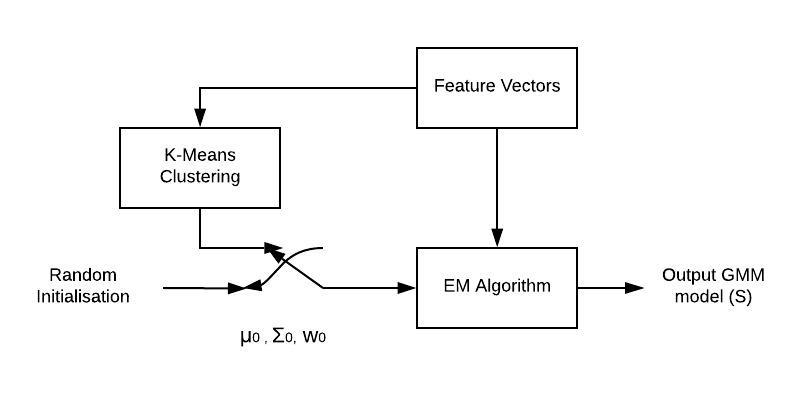
\includegraphics[scale=.65]{Images/gmm_em.jpeg}}
\caption{Basic block diagram of GMM training.}
\label{gem}
\end{figure} 
\subsubsection{Expectation Maximization Algorithm}

We have to maximize the likelihood $L(X|S)$ with respect to the model parameters $S=\{w_{i},\mu_{i},\Sigma_{i}\}$, then the partial derivative with respect to $\mu_{i}$ and $\Sigma_{i}$ can be written as:

\begin{equation}
\begin{aligned}
\label{lpd}
 \frac{\partial L(X|S)}{\partial \mu_{i}}=&\frac{\sum_{j=1}^{T} w_{i}P(x_{j}|\theta_{i})\Big(\frac{x_{j}-\mu_{i}}{\Sigma_{i}}\Big)}{\sum_{i=1}^{M_{g}} w_{i}P(x_{j}|\theta_{i})}\\
 \frac{\partial L(X|S)}{\partial \Sigma_{i}}=&\frac{\sum_{j=1}^{T} w_{i}P(x_{j}|\theta_{i})\Big(\frac{\Sigma_{i}^{-1}(x_{j}-\mu_{i})(x_{j}-\mu_{i})^{T}\Sigma_{i}^{-1}}{2}-\frac{1}{2\Sigma_{i}}\Big)}{\sum_{i=1}^{M_{g}} w_{i}P(x_{j}|\theta_{i})}, \quad i=1,2,\ldots,M_{g}
 \end{aligned}
\end{equation}

Equating the partial derivatives in the equation~\ref{lpd} to zero and by assuming,
\begin{equation}
\label{gm}
    \gamma_{ij}=\frac{w_{i}P(x_{j}|\theta_{i})}{{\sum_{i=1}^{M_{g}} w_{i}P(x_{j}|\theta_{i})}}
\end{equation}

the $\mu_{i}$ and $\Sigma_{i}$ can be written as:

\begin{equation}
\begin{aligned}
\label{opmv}
\mu_{i}=&\frac{\sum_{j=1}^{T}\gamma_{ij}x_{j}}{\sum_{j=1}^{T}\gamma_{ij}}\\
\Sigma_{i}=&\frac{\sum_{j=1}^{T}\gamma_{ij}(x_{j}-\mu_{i})(x_{j}-\mu_{i})^{T}}{\sum_{j=1}^{T}\gamma_{ij}}, \quad i=1,2,\ldots,M_{g}
\end{aligned}
\end{equation}

%
There is a constraint of $\sum_{i=1}^{M_{g}}w_{i}=1$, so to find the optimal value, we have to use Lagrange constraint optimization, the modified objective function can be written as:
\begin{equation}
\label{obj}
    \max_{w_{i}} \quad L(X|S)+\eta \Bigg(\sum_{i=1}^{M_{g}}w_{i}-1 \Bigg)
\end{equation}

The partial derivative of equation~\ref{obj} with respect to $w_{i}$ can be written as:
\begin{equation}
\begin{aligned}
\label{wop}
\frac{\partial \Bigg(L(X|S)+\eta \Bigg(\sum_{i=1}^{M_{g}}w_{i}-1 \Bigg)\Bigg)}{\partial w_{i}}=&\sum_{j=1}^{T}\frac{P(x_{j}|\theta_{i})}{\sum_{i=1}^{M_{g}} w_{i}P(x_{j}|\theta_{i})}\\
 =&\sum_{j=1}^{T} \frac{\gamma_{ij}}{w_{i}}+\eta\\
\end{aligned}
\end{equation}
Equating the partial derivatives in the equation~\ref{wop} to zero, 

\begin{equation}
\label{lsl}
    \begin{aligned}
     \sum_{j=1}^{T}\gamma_{ij}=&-\eta(w_{i})\\
     -\eta (w_{1}+w_{2}+\ldots+w_{M_{g}})=&\sum_{i=1}^{M_{g}}\sum_{j=1}^{T}\gamma_{ij}\\
    - \sum_{i=1}^{M_{g}}\sum_{j=1}^{T}\gamma_{ij}=&\eta \quad \quad  \Bigg(as \quad \sum_{i=1}^{M_{g}}w_{i}=1\Bigg)
    \end{aligned}
\end{equation}

From the definition of $\gamma_{ij}$ (as per equation~\ref{gm}) we can say, $\gamma_{ij}$ is the probability of $j^{th}$ vector corresponds to $i^{th}$ Gaussian. So, $\sum_{i=1}^{M_{g}}\gamma_{ij}=1$, and $\sum_{j=1}^{T}\sum_{i=1}^{M_{g}}\gamma_{ij}=T$.

From equation~\ref{lsl}, we get $\eta = -T$, and $w_{i}$ can be written as:
\begin{equation}
w_{i}=\frac{1}{T}\sum_{j=1}^{T}\gamma_{ij}
\end{equation}

Putting all together, we can write the estimated values of $w_{i},\mu_{i}$, and $\Sigma_{i}$ as:
\begin{equation}
\begin{aligned}
\label{op}
\mu_{i}=&\frac{\sum_{j=1}^{T}\gamma_{ij}x_{j}}{\sum_{j=1}^{T}\gamma_{ij}}\\
\Sigma_{i}=&\frac{\sum_{j=1}^{T}\gamma_{ij}(x_{j}-\mu_{i})(x_{j}-\mu_{i})^{T}}{\sum_{j=1}^{T}\gamma_{ij}}\\
w_{i}=&\frac{1}{T}\sum_{j=1}^{T}\gamma_{ij}, \quad i=1,2,\ldots,M_{g}\\
where, \quad \gamma_{ij}=&\frac{w_{i}P(x_{j}|\theta_{i})}{{\sum_{i=1}^{M_{g}} w_{i}P(x_{j}|\theta_{i})}}
\end{aligned}
\end{equation}
From the above equation~\ref{op}, It is worth to note that the results don't constitute a close form solution. The parameters of the GMM depends on $\gamma_{ij}$ value, which again depends on the model parameters. This suggests, solve for a analytic solution is not possible. The solution can be obtain by using a simple iterative procedure. Which is well known as EM algorithm. We first choose some initial values for the means, covariances, and weights. Then by considering the initial values, the $\gamma_{ij}$ value is computed (known as expectation step) and then using the $\gamma_{ij}$ value the means, covariances, and weights values are computed (known as maximization step). The equation~\ref{op} can be modified as:

\begin{equation}
\begin{aligned}
\label{opi}
\gamma_{ij}^{k+1}=&\frac{w_{i}^{k}P(x_{j}|\theta_{i}^{k})}{{\sum_{i=1}^{M_{g}} w_{i}^{k}P(x_{j}|\theta_{i}^{k})}}\\
\mu_{i}^{k+1}=&\frac{\sum_{j=1}^{T}\gamma_{ij}^{k+1}x_{j}}{\sum_{j=1}^{T}\gamma_{ij}^{k+1}}\\
\Sigma_{i}^{k+1}=&\frac{\sum_{j=1}^{T}\gamma_{ij}^{k+1}(x_{j}-\mu_{i}^{k+1})(x_{j}-\mu_{i}^{k+1})^{T}}{\sum_{j=1}^{T}\gamma_{ij}^{k+1}}\\
w_{i}^{k+1}=&\frac{1}{T}\sum_{j=1}^{T}\gamma_{ij}^{k+1}, \quad i=1,2,\ldots,M_{g}\\
\end{aligned}
\end{equation}

The process continues until $L(X|S^{k+1}) \geq L(X|S^{k})$. In general the EM algorithm takes many more iteration for convergence, thus K-means algorithm is used to initialize the model parameters. For each observation X, if the $\gamma_{ij}$ value is given, than its known as complete data, in such cases the analytic solution can be obtained using equation~\ref{op}. But, in practice only observations are given known as incomplete data. In such situation, EM algorithm is used to estimate the model parameters.  
\subsubsection{Maximum a posteriori (MAP) Parameter estimation}
\label{secmap}
The parameters of the GMM can also be estimated using MAP estimation. This approach is generally used in the pattern recognition tasks where the available labeled training data is limited. In speaker and language recognition task this approach is used to derive the adapted speaker/language model by adapting the training vectors with the universal background model (UBM)~\cite{reynolds2000speaker}. 

Like EM algorithm, the MAP estimation is also a two step process.
\begin{enumerate}
    \item Step 1: The sufficient statistics of the training data are computed for each mixture in the prior model (The model computed using ML estimation).
    \item Step 2: The new estimated sufficient statistics are combined with the old sufficient statistics sufficient statistics from the prior mixture parameters using a data-dependent mixing coefficient. 
\end{enumerate}
The data-dependent mixing coefficient is designed so that mixtures with high counts of new data rely more on the new sufficient for final parameter estimation and mixtures with low counts of new data rely more on the old sufficient statistics for final parameter estimation. The prior model is a large GMM (known as UBM) that is trained using ML estimation with large amount of data which encompasses the different kinds of speech that may be encountered by the system during training. These different kinds may include different channel conditions, composition of speakers/languages, acoustic conditions, etc.

Given a prior model ($S^{prior}$) and training vectors from the desired class ($X=\{x_{1},x_{2},\ldots,x_{T}\}$), the sufficient statistics with respect to the prior model can be computed using equation~\ref{s1map}.

\begin{equation}
\label{s1map}
    \begin{aligned}
     \gamma_{ij}=&\frac{w_{i}^{prior}P(x_{j}|\theta_{i}^{prior})}{\sum_{i=1}^{M_{g}}w_{i}^{prior}P(x_{j}|\theta_{i}^{prior})}\\
     n_{i}=&\sum_{j=1}^{T}\gamma_{ij}\\
     E_{i}(X)=&\frac{1}{n_{i}}\sum_{j=1}^{T}\gamma_{ij}x_{j}\\
     E_{i}(X^{2})=&\frac{1}{n_{i}}\sum_{j=1}^{T}\gamma_{ij}~\mbox{Diag}(x_{j}x_{j}^{T})
    \end{aligned}
\end{equation}

The new sufficient statistics computed from the training data then used to update the prior sufficient statistics for mixture $i$ to create the adapted parameters for mixture $i$ by using the equation~\ref{s2map} 
\begin{equation}
\label{s2map}
    \begin{aligned}
     \hat{w_{i}}=&\Bigg[\frac{\alpha_{i}^{w}n_{i}}{T}+(1-\alpha_{i}^{w})w_{i}\Bigg]\Gamma\\
     \hat{\mu_{i}}=&\alpha_{i}^{m}E_{i}(x_{t})+(1-\alpha_{i}^{m})\mu_{i}\\
      \hat{\Sigma_{i}}=&\alpha_{i}^{v}E_{i}(x_{t}^{2})+(1-\alpha_{i}^{v})(\mbox{Diag}~( \Sigma_{i})+\mu_{i}^{2})-\hat{\mu_{i}}^{2}
    \end{aligned}
\end{equation}
 A scale factor $\Gamma$ is used, which ensures that all the new mixture weights sum to 1. $\alpha_{i}^{w},\alpha_{i}^{m}$ and $\alpha_{i}^{v}$ are the adaptation coefficient which controls the balance between the old and new model parameter estimates. $\alpha_{i}$ is defined as:
 \begin{equation}
   \alpha_{i}^{w}=\alpha_{i}^{m}= \alpha_{i}^{v}=\alpha_{i}=\frac{n_{i}}{n_{i}+r}
 \end{equation} 
 \begin{figure}[h]
\centering{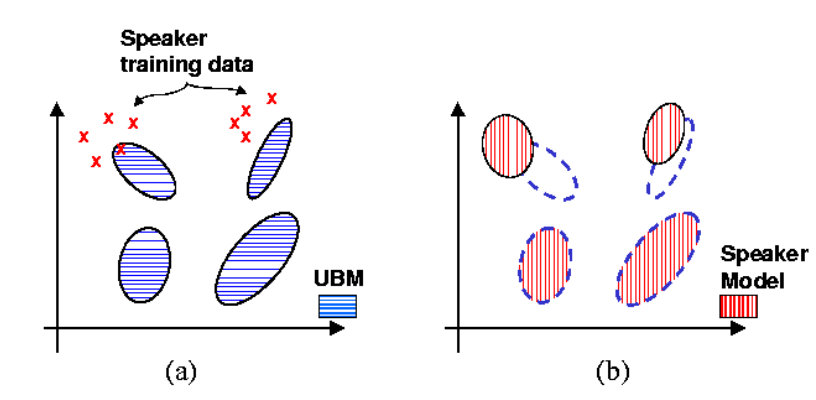
\includegraphics[scale=.45]{Images/MAP.png}}
\caption{(a) The training vectors (x’s) are probabilistically mapped
into the UBM (prior) mixtures. (b) The adapted mixture parameters are derived using the statistics of the new data and the UBM (prior) mixture parameters. The adaptation is data dependent, so UBM (prior) mixture parameters are adapted by different amounts~\cite{reynolds1995speaker}.}
\label{map}
\end{figure}
 where r is a fixed relevance factor, which determines the extent of mixing of the old and new estimates of the parameters. If a mixture component has a low probabilistic count ($n_{i}$) of new data, then $\alpha_{i}\Rightarrow 0$ causing the de-emphasis of the new (potentially under-trained) parameters and the emphasis of the old (better trained) parameters. For mixture components with high probabilistic counts, $\alpha_{i}\Rightarrow 1$ causing the use of the new class-dependent parameters. The pictorial representation of the same is presented in figure~\ref{map}. The relevance factor is a way of controlling how much new data should be observed in a mixture before the new parameters begin replacing the old parameters. Thus, this approach is robust to limited training data.
 

 \subsection{Testing of GMMs}
\begin{figure}[h]
\centering{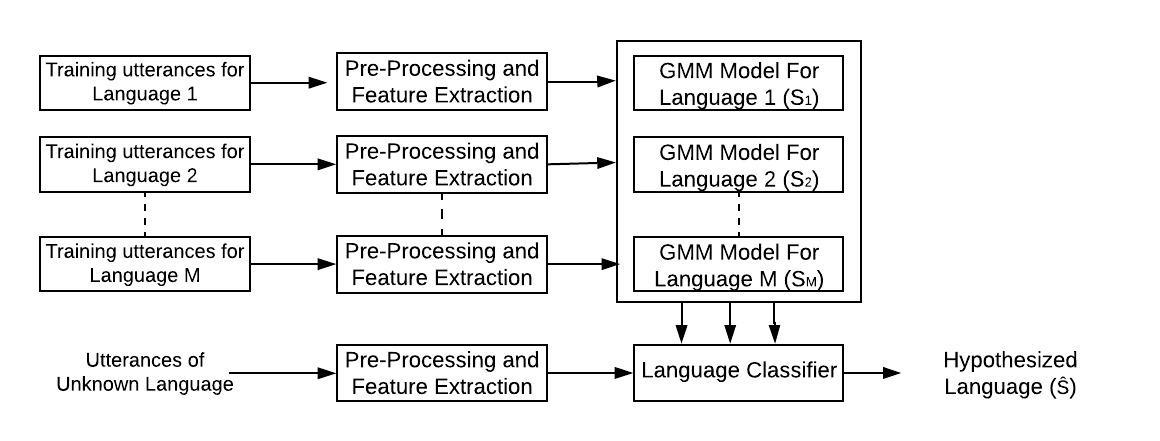
\includegraphics[scale=.65]{Images/gmm.jpeg}}
\caption{Basic block diagram of language identification using GMM.}
\label{gmm}
\end{figure} 

 In the testing phase the objective is to identify the hypothesized model from a set of models $\{S_{1}, S_{2},...,S_{M}\}$ given a set of testing vectors $X=\{x_{1}, x_{2},.., x_{T}\}$. The identified model ($\hat{S}$) can be evaluated using equation~\ref{tllk}. 

\begin{equation} 
\begin{aligned}
\label{tllk}
\hat{S} =&\mbox{arg}~\max_{1 \leq i \leq M} P(S_{i}|X)\\
        =&\mbox{arg}~\max_{1 \leq i \leq M} \frac{P(X|S_{i})}{P(X)}P(S_{i})
\end{aligned}
\end{equation}
 Using ML detection criteria (i.e Assuming equal probability occurrence of all the models )  and the statistical independence of the testing vectors, the decision rule for the most probable model can be redefined as:
 \begin{equation}
  \hat{S}=\mbox{arg}~\max_{1 \leq i \leq M}\sum_{j=1}^{T}~\mbox{log}(P(x_{j}|S_{i}))
 \end{equation} 

The basic block diagram of Language identification task using GMM based training and testing are presented in figure~\ref{gmm}. 

\section{Gaussian Mixture Model and Universal Background Model (GMM-UBM)}
\label{cgmmubm}

The GMM-UBM approach is a vary successful technique for speaker recognition applications. Later by inspiring from the performance of GMM-UBM based speaker recognition systems, people start using GMM-UBM technique in language identification task. After GMM-UBM technique dominantly used in language identification task.
\begin{figure}[h]
\centering{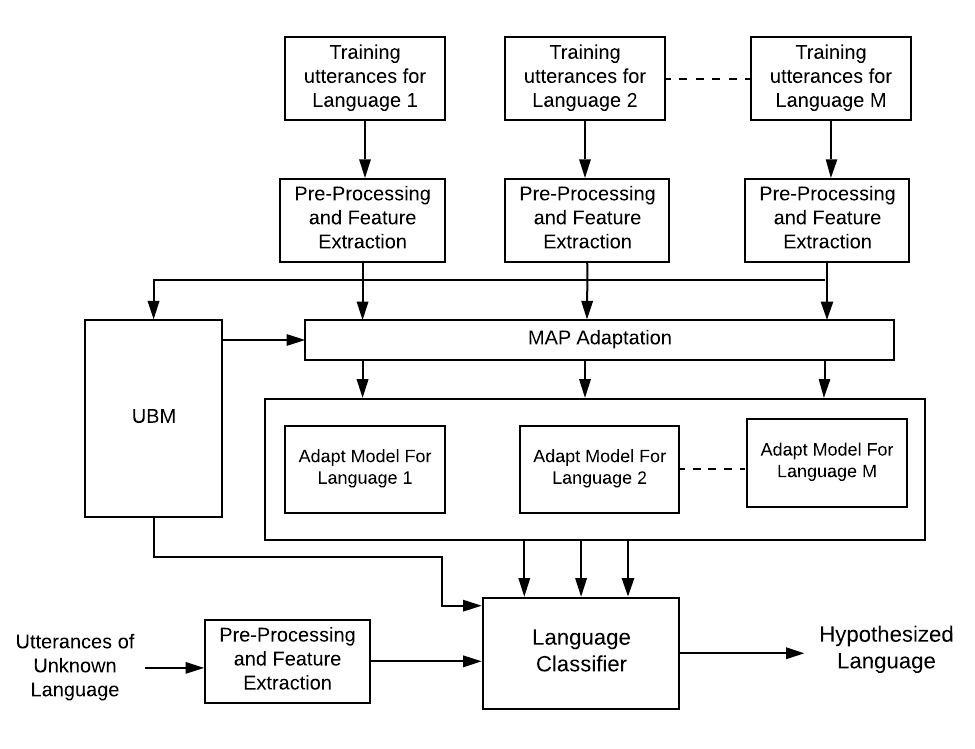
\includegraphics[scale=.65]{Images/ubm.jpeg}}
\caption{Basic block diagram of language identification using GMM-UBM.}
\label{ubm}
\end{figure}

The basic block diagram of GMM-UBM based language identification system is shown in figure~\ref{ubm}. The training phase of GMM-UBM technique is divided into two distinct stages. First a set of feature vector from a number of different languages (typically data from all possible languages used for testing) are taken to train a single GMM (known as UBM). The UBM is considered to represent the characteristics of all different languages. In the second stage the UBM is adapted for each of the languages in the system using MAP adaptation. The detail of MAP adaptation training procedure is described in section~\ref{secmap}. The idea behind MAP adaptation is that, the parameters of the Gaussian which show higher probability towards the language training data will tends towards the parameters of the training data, and the parameters of the mixture show lower probability to the language training data will remain fairly close to the original UBM. The MAP adaptation of the GMM parameters is often applied to the means of the mixture components rather than means, variances and weights (i.e. $\alpha^{v},\alpha^{w}=0$)~\cite{ambikairajah2011language}.      

In the testing phase, given a set of testing vectors $\{x_{1},x_{2},\ldots,x_{T}\}$ , UBM model $S^{ubm}$ and the adapt models of each language $\{S_{i}^{adapt}\}_{i=1}^{M}$, the identified language model can be evaluated using equation~\ref{gmmubmeva}. Where $M$ is the total no of languages used in the system.

\begin{equation}
    \label{gmmubmeva}
   \hat{S}=\mbox{arg}~\max_{1 \leq i \leq M}\sum_{j=1}^{T}\bigg[~\mbox{log}(P(x_{j}|S_{i}^{adapt})) - ~\mbox{log}(P(x_{j}|S^{ubm})\bigg]
\end{equation}

\section{I-vector based language identification system}
\label{ivector}
Language recognition and speaker recognition has many similarities in terms of technical formulation. Thus, in literature most of the descriptors and modeling techniques used to perform language identification task are borrowed from speaker recognition. In case of speaker recognition, in GMM-UBM based statistical modeling, the MAP adaptation not only adapt the speaker specific information but also adapts the channel and session variations. Thus to improve the speaker recognition performance, needs a modeling technique which can model the speaker specific information and other variability separately or to model all the information, suppress the other variability and retain the speaker specific information. In~\cite{kenny2005joint}, the authors propose a method to model all the variations separately. They represented a speaker utterance by a supervector (M), that consists of additive components of speaker and channel/session subspace. This technique is well known as joint factor analysis (JFA).  The speaker dependent supervector is defined as:
\begin{equation}
    \label{jfa}
    M=m+Vy+Ux+Dz
\end{equation}
where m is a speaker and session independent supervector (generally mean vector of UBM having $M_{g}D\times 1$ dimension). $V$ and $D$ define a speaker subspace (eigenvoice matrix and diagonal residual respectively), and $U$ defines a session or channel subspace (eigen channel matrix). The vector $y$, $z$ and $x$ are the speaker and channel/session dependent factors in their respective subspace and each is assumed to be a random variable with a standard normal distribution ($N(0,I)$). In JFA, first the subspaces (i.e $V$, $D$ and $U$) have to be estimated from the appropriate labeled corpora, than the speaker and session factors (i.e $y$, $z$ and $x$) have to be computed for the target utterances. The scoring is done by computing the likelihood of the test utterance vectors against the session compensated speaker model ($M-Ux$). In~\cite{dehak2011front}, the authors slightly modify the modeling technique to reduce the computation and enhance the recognition performance. The authors proposed a single subspace modeling instead of two subspace (speaker and channel separately). This single subspace is known as total variability subspace. The total variability subspace contains both the speaker and channel variability information. The new speaker and channel dependent supervector can be  defined as:
\begin{equation}
    \label{ivec}
    M=m+Tw
\end{equation}
where $T$ is the total variability subspace and $w$ is the speaker and channel dependent vector (known as identity vector/ i-vector). $T$ is a rectangular matrix of low rank and $w$ is a vector having standard normal distribution. After i-vector extraction some channel compensation techniques (like linear discriminative analysis (LDA), within class covariance normalization (WCCN) and nuisance attribute projection (NCA)) are used to suppress the channel variability. A cosine kernel scoring technique is used to find the recognition performance. The block diagram of i-vector based language recognition system is shown in figure ~\ref{i-vec}. 

\begin{figure}[h]
\centering{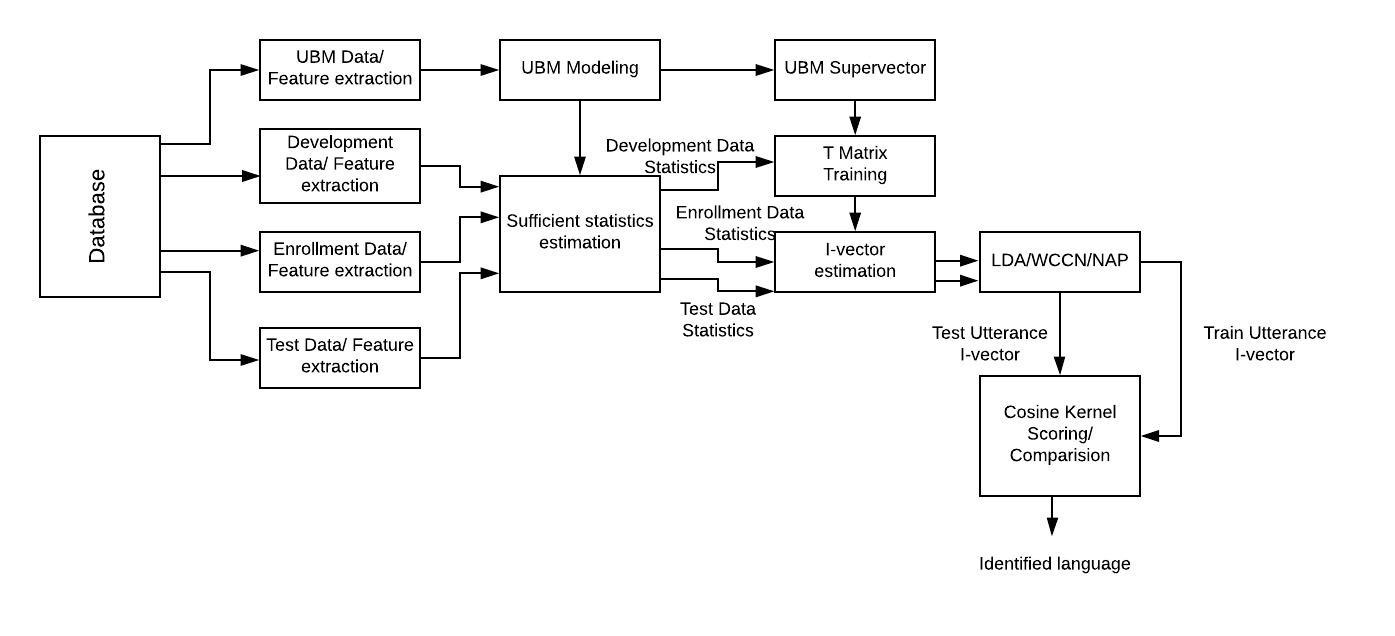
\includegraphics[scale=.65]{Images/i_vector.jpeg}}
\caption{Basic block diagram of language identification using i-vector.}
\label{i-vec}
\end{figure}
From the figure~\ref{i-vec}, it has been seen that, the whole dataset is segmented into four parts: UBM data, development data, enrollment data, test data. UBM data consists of data of all the languages, used to build UBM models as described in section~\ref{cgmmubm}. The development data segment also consists of utterances from all the languages, used to estimate the total variability matrix. After the estimation of total variability matrix (T matrix), the hidden variable $w$, known as i-vector is estimated from each utterance of the enrollment and test data. The i-vector $w$, which can be defined by its posterior distribution conditioned to the Baum-Welch statistics for a given utterance. The posterior distribution is a Gaussian distribution and the Baum-Welch sufficient statistics will be estimated from the UBM. Suppose we have $T$ frames $\{x_{1}, x_{2}, \ldots, x_{T}\}$ of an utterance and the UBM composed of $M_{g}$ mixture components defined in some feature space of dimension $D$. The Sufficient statistics for a given utterance is given by:
\begin{equation}
    \begin{aligned}
     N_{i}=&\sum_{j=1}^{T}\gamma_{ij} \quad (zeroth ~order ~statistics)\\
     F_{i}=&\sum_{j=1}^{T}\gamma_{ij}x_{j} \quad (first ~order ~statistics)\\
     S_{i}=&\mbox{diag}\Bigg[\sum_{j=1}^{T}\gamma_{ij}x_{j}x_{j}^{*}\Bigg], \quad i=1,2,\ldots,M_{g} \quad (second ~order ~statistics)
    \end{aligned}
\end{equation}
where $x_{j}^{*}$ is the Hermitian transpose of vector $x_{j}$ and $\gamma_{ij}=\frac{w_{i}P(x_{j}|\theta_{i})}{{\sum_{i=1}^{M_{g}} w_{i}P(x_{j}|\theta_{i})}}$ (from equation~\ref{gm}).  In order to estimate the i-vector, we need to centralize the first and second order sufficient statistics. The centralized statistics is given by:
\begin{equation}
    \begin{aligned}
     \tilde{F}_{i}=&\sum_{j=1}^{T}\gamma_{ij}(x_{j}-m_{i}) \\
        =&\sum_{j=1}^{T}\gamma_{ij}x_{j}-\sum_{j=1}^{T}\gamma_{ij}m_{i}\\
        =&F_{i} - N_{i}m_{i}\\
     \tilde{S_{i}}=&\mbox{diag}\Bigg[\sum_{j=1}^{T}\gamma_{ij}(x_{j}-m_{i})(x_{j}-m_{i})^{*}\Bigg], \quad i=1,2,\ldots,M_{g}\\
     =& S_{i}-\mbox{diag}(F_{i}m_{i}^{*}+m_{i}F_{i}^{*}-N_{i}m_{i}m_{i}^{*})
    \end{aligned}
\end{equation}
where $m_{i}$ is the mean vector of the $i^{th}$ mixture. We can write the statistics in the matrix format as:
\begin{equation}
    \begin{aligned}
     N_{m}=&\begin{bmatrix} 
        N_{1}*I &     &                 \\
                &\ddots&                \\
                &       & N_{M_{g}}*I 
        \end{bmatrix}\\
    F_{m}=&\begin{bmatrix}
            \tilde{F}_{1}\\
            \vdots      \\
            \tilde{F}_{M_{g}}
            \end{bmatrix}\\
    S_{m}=&\begin{bmatrix} 
        \tilde{S}_{1} &     &                 \\
                &\ddots&                \\
                &       & \tilde{S}_{M_{g}} 
        \end{bmatrix}\\        
    \end{aligned}
\end{equation}
where $N_{m}$ is a matrix of dimension $M_{g}D \times M_{g}D$, $I$ is a identity matrix of dimension $D \times D$, $F_{m}$ is a  vector of dimension $M_{g}D \times 1$ and $S_{m}$ is a matrix of dimension $M_{g}D \times M_{g}D$. In~\cite{kenny2005joint} from Theorem 2 we can write the distribution of the hidden variable (w) is $N(L_{T}^{-1}*T^{*}*\Sigma^{-1}*F_{m},L_{T}^{-1})$. The i-vector can be computed as $E(w)=L_{T}^{-1}*T^{*}*\Sigma^{-1}*F_{m}$. where $E(w)$ is the expectation of vector $w$, $\Sigma$ is the variance of the UBM, $L_{T}= I+T^{*}\Sigma^{-1}N_{m}T$ and $T$ is the total variability matrix.

\subsection{T Matrix training}
\begin{enumerate}
    \item Step 1: Initialize the T matrix randomly having dimension $M_{g}D \times Dimension~of~i-vector$
    \item Step 2: Compute: $L_{T}=I+T^{*}\Sigma^{-1}*N_{m}*T$
    \item Step 3: Accumulate the statistics across utterances:
    \begin{equation}
        \begin{aligned}
         ^{a}N_{i}=&\sum_{u}N_{i}(u)\\
         ^{a}A_{i}=&\sum_{u}N_{i}(u)L_{T}^{-1}\\
         ^{a}C=&\sum_{u}F_{m}(u)(L_{T}^{-1}(u)*T^{*}*\Sigma^{-1}*F_{m}(u))\\
         ^{a}N_{m}=&\sum_{u}N_{m}(u)
        \end{aligned}
    \end{equation}

    \item Step 4: Compute T matrix:
    \begin{equation}
        T=\begin{bmatrix}
        T_{1}\\
        \vdots\\
        T_{M_{g}}
        \end{bmatrix}=\begin{bmatrix}
        A_{1}^{-1}*C_{1}\\
        \vdots\\
        A_{M_{g}^{-1}*C_{M_{g}}}
        \end{bmatrix}, \quad where \quad C=\begin{bmatrix}
        C_{1}\\
        \vdots\\
        C_{M_{g}}
        \end{bmatrix}
    \end{equation}
    \item Step 5: Compute covariance update (optional):
    \begin{equation}
        \Sigma= (^{a}N_{m})^{-1}\Bigg[\sum_{u}S_{m}(u)-\mbox{diag}(C*T^{*})\Bigg]
    \end{equation}
    \item Step 6: Iterate step 2 to step 4 (or step 5) approximately 20 times to get the estimate of the T matrix.
\end{enumerate}
In the literature, people have not used the second order statistics($S_{m}$) for speaker and language recognition task, in such cases step 5 is not required.
 \subsection{I-vector estimation}
 After the estimation of T matrix the i-vectors from each utterances of the enrollment set and test set is computed using equation~\ref{eivec}.
 \begin{equation}
 \label{eivec}
    w(u)= L_{T}^{-1}(u)*T^{*}*\Sigma^{-1}*F_{m}(u)
 \end{equation}
 
 \subsection{Cosine kernel scoring}
 Cosine kernel scoring is technique to find the cosine kernel between the train language i-vectors and test i-vector. Suppose there are L languages having each $K_{1},K_{2}, \ldots, K_{L}$ utterances and lets denote the train language i-vector as $w_{lk}$ and the test utterance i-vector as $w_{test}$. The identified language ($\hat{S}$) can be written as
 
 \begin{equation}
     \hat{S}=\mbox{arg}~\max_{1 \leq l \leq L} \sum_{k=1}^{K_{l}} Score_{lk}=\mbox{arg}~\max_{1 \leq l \leq L} \sum_{k=1}^{K_{l}} \frac{<w_{lk},w_{test}>}{||w_{lk}||||w_{test}||}
 \end{equation}
 
 \subsection{Intersession compensation techniques}
 \label{lda}
 The intersession compensation techniques are used to enhance the inter-class variations and to suppress the intra-class variations.  Generally there are three dominantly used intersession compensation technique to enhance the recognition performance, while the classes are modeled in total variability space. These three techniques are: linear discriminant analysis (LDA), within class covariance normalization (WCCN), nuisance attribute projection (NAP). 
 \subsubsection{Linear discriminant analysis (LDA)}
 LDA is a technique of dimensionality reduction, widely used in the task of pattern recognition. The motivation of using LDA in i-vector based language recognition task is that, as all the utterances of a given language are assume to represent one class, LDA attempts to define new special axes that minimize the intra-class variance caused by channel and speaker effects, and to maximize the variance between languages. This approach searches a new orthogonal axes to better discriminate between classes. The LDA optimization problem can be defined according to the ratio given in equation~\ref{ld1}. 
 \begin{equation}
     \label{ld1}
     J(v)=\frac{v^{t}S_{b}v}{v^{t}S_{w}v}
 \end{equation}
 The ratio is often referred as the Rayleigh coefficient for space direction $v$. $S_{b}$ and $S_{w}$ are the between class and the within-class variance between matrix and are calculated as follows:
 \begin{equation}
 \begin{aligned}
   S_{b}=&\sum_{l=1}^{L}(w_{l}-\bar{w})(w_{l}-\bar{w})^{t}\\
   S_{w}=&\sum_{l=1}^{L}\frac{1}{K_{L}}\sum_{k=1}^{K_{L}}(w_{k}^{l}-\bar{w}_{l})(w_{k}^{l}-\bar{w}_{l})^{t}
 \end{aligned}
 \end{equation}
 where $\bar{w}_{l}=\frac{1}{K_{L}}\sum_{k=1}^{K_{L}}w_{k}^{l}$ is the mean of i-vectors for each language. $\bar{w}$ is the mean of i-vector for all the utterances. The maximization is used to define a projection matrix A composed by the best eigen vectors (those with highest eigen values) of the general eigen value equation:
 \begin{equation}
     \begin{aligned}
      S_{b}v=&\lambda S_{w}v\\
      S_{b}S_{w}^{-1}v=&\lambda v
     \end{aligned}
 \end{equation}
 where $\lambda$ is the diagonal matrix of eigenvalues. The the projection matrix is obtained by taking the eigen vectors of the larger eigenvalues (i.e $A=V(:,1:no~of~top~eigen~values)$).The identified language ($\hat{S}$) can be written as:
 
 \begin{equation}
     \hat{S}=\mbox{arg}~\max_{1 \leq l \leq L} \sum_{k=1}^{K_{l}} Score_{lk}=\mbox{arg}~\max_{1 \leq l \leq L} \sum_{k=1}^{K_{l}} \frac{<A^{t}w_{lk},A^{t}w_{test}>}{||A^{t}w_{lk}||||A^{t}w_{test}||}
 \end{equation}
  
  \subsubsection{Within class covariance normalization (WCCN)}
  This technique was first introduced in~\cite{hatch2006within}. In the study, they applied this approach in SVM modeling based on linear separation between target speaker and imposter using one verses all decision. WCCN techniques uses inverse of within-class covariance to normalize the cosine kernel. The resulting solution by a generalized linear kernel form can be written as given in ~\cite{hatch2006within}:
  \begin{equation}
      k(w_{1},w_{2})=w_{1}^{t}Rw_{2}
  \end{equation}
  where $R$ is a symmetric positive semi-definite matrix. The optimal normalized kernel matrix is given by $R=W^{-1}$. W is a within class covariance matrix, calculated as:
  \begin{equation}
      W=\frac{1}{L}\sum_{l=1}^{L}\frac{1}{K_{L}}\sum_{k=1}^{K_{L}}(w_{k}^{l}-\bar{w}_{l})(w_{k}^{l}-\bar{w}_{l})^{t}
  \end{equation}
  In order to preserve the inner product form of the cosine kernel, a feature-mapping function $\varphi$ can be defined as:
  \begin{equation}
      \varphi(w)=B^{t}w
  \end{equation}
  where B is obtained through Cholesky decomposition of matrix $W^{-1}=BB^{t}$. The WCCN algorithm uses the within-class covariance matrix to normalize the cosine kernel function to normalize the cosine kernel functions in order to compensate for intersession variability, while guaranteeing conservation of directions in space. The identified language ($\hat{S}$) can be written as:
 
 \begin{equation}
     \hat{S}=\mbox{arg}~\max_{1 \leq l \leq L} \sum_{k=1}^{K_{l}} Score_{lk}=\mbox{arg}~\max_{1 \leq l \leq L} \sum_{k=1}^{K_{l}} \frac{<B^{t}w_{lk},B^{t}w_{test}>}{||B^{t}w_{lk}||||B^{t}w_{test}||}
 \end{equation} 
 
 \subsubsection{Nuisance attribute projection (NAP)}
 The nuisance attribute projection algorithm is presented in~\cite{campbell2006svm}. It is based on finding an appropriate projection matrix intended to remove the nuisance direction. The projection matrix carries out an orthogonal projection in channel's and speaker's complimentary space, which depends only on language class information. The projection matrix is formulated as:
 \begin{equation}
     P=I-RR^{t}
 \end{equation}
 where $R$ is a rectangular matrix of low rank, whose columns are the eigen vectors ($Wr=\lambda r$) having the best eigen values of the within-class covariance matrix (W) computed as:
  \begin{equation}
      W=\frac{1}{L}\sum_{l=1}^{L}\frac{1}{K_{L}}\sum_{k=1}^{K_{L}}(w_{k}^{l}-\bar{w}_{l})(w_{k}^{l}-\bar{w}_{l})^{t}
  \end{equation}
   
 The identified language ($\hat{S}$) using NAP can be written as:
 
 \begin{equation}
     \hat{S}=\mbox{arg}~\max_{1 \leq l \leq L} \sum_{k=1}^{K_{l}} Score_{lk}=\mbox{arg}~\max_{1 \leq l \leq L} \sum_{k=1}^{K_{l}} \frac{<P^{t}w_{lk},P^{t}w_{test}>}{||P^{t}w_{lk}||||P^{t}w_{test}||}
 \end{equation} 



\section{Feedforward network based model}
\label{ffnn}
\begin{figure}[h]
\centering{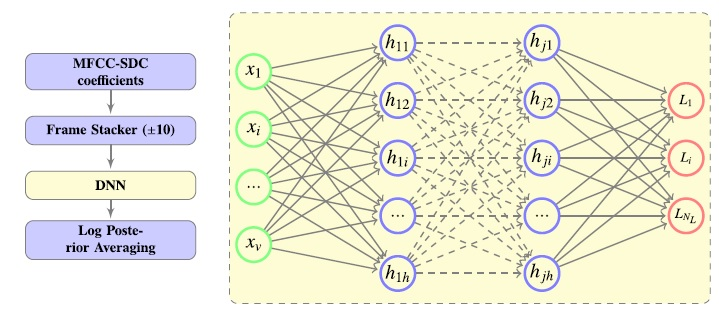
\includegraphics[scale=.65]{Images/ffn.jpg}}
\caption{Feedforward network based classifier~\cite{lopez2016use}.}
\label{ffn}
\end{figure}

The impressive gain in performance obtained using deep neural networks (DNNs) for automatic speech recognition (ASR) have motivated the application of DNNs in other speech technologies such as language recognition and speaker recognition. Feedforward neural network is a fully connected network, which shows the direct use of DNN in the recognition task. In this approach, a fully connected network with multiple hidden layers is trained using back-propagation algorithm to perform recognition task. The output layer of this network has the number of neurons (nodes) same as the number of classes in the recognition task, whereas the input layer has the number of nodes same as the dimension of input feature vector (refer figure~\ref{ffn}). In general, the MFCC/SDC features are computed and then stacked with the feature vectors of the neighboring frames and then given input to the network.  After training is over, testing is performed using the feature vectors of the speech utterances.  For a test utterance, the output score is computed as:
\begin{equation}
    score_{l}=\frac{1}{N}\sum_{t=1}^{N}log p(L_{l}|x_{t},\Theta)
\end{equation}
where $p(L_{l}|x_{t},\Theta)$ represents the class probability output for language l corresponding to the input example at time $t$, $x_{t}$ is the feature vector and $\Theta$ is the parameter of the DNN.

For a test utterance, the output node giving the highest score is termed as the recognition class.  





\section{Bottleneck feature I-vector model}
DNN architectures can be used for feature extraction. From the human language recognition ability, it has been seen that both acoustic phonetic and phonotactic information are used for recognition. Thus people try to extract the features, which have both the information. This type of feature can be extracted by training a DNN, by providing the feature vector to the input and its corresponding posterior senone probabilities (computed from a DNN based ASR system) to the output of the DNN. After the network is trained, activation value of a hidden layer near to output layer can be taken as a feature vector (known as bottleneck feature (BNF)) by providing acoustic feature vectors as input(refer figure~\ref{bnf}). After the BNF feature is extracted, I-vector framework is used to identify the language( refer to figure~\ref{bnf1}).  
\begin{figure}[h]
\centering{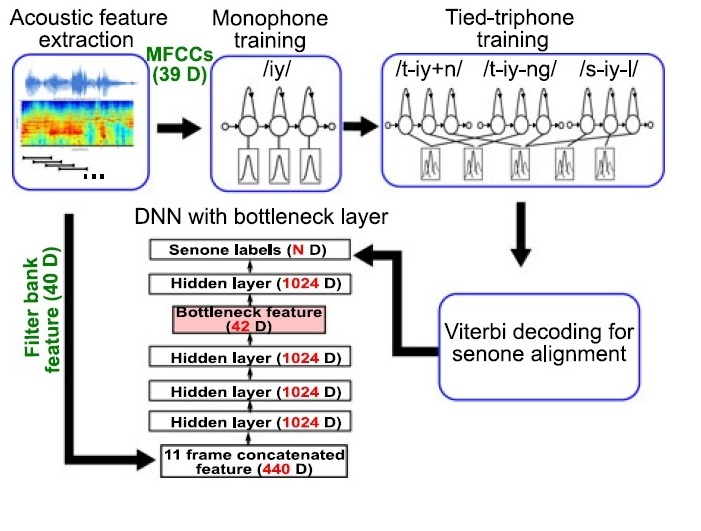
\includegraphics[scale=.30]{Images/dnn_i_vector1.jpg}}
\caption{Bottleneck feature extraction~\cite{zhang2018language}.}
\label{bnf}
\end{figure}
\begin{figure}[h]
\centering{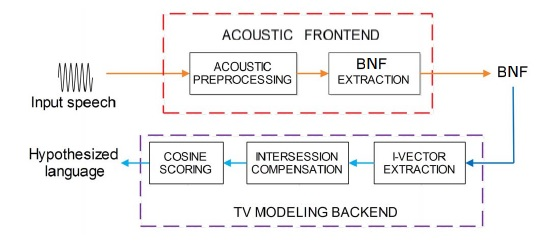
\includegraphics[scale=.60]{Images/bnf.jpg}}
\caption{Bottleneck feature-I-vector based language identification system~\cite{jiang2014deep}.}
\label{bnf1}
\end{figure}

\section{X-vector based modeling}
\label{xvector}
In this approach, the X-vectors are extracted from a trained DNN and then used like I-vectors to perform recognition task. The DNN is trained to discriminate between languages/speakers. The X-vector is a fixed dimensional embedding extracted from the variable length utterance, using a trained time delay neural network (TDNN) based DNN. TDNN is a older approach proposed in~\cite{waibel1989phonemetdnn} on 1989. TDNN works like convolutional neural network (CNN) work on the image to capture local information. The disadvantage of TDNN is, it requires a high amount of data and training time. Thus, in this approach, a subsampling method is used on TDNN to reduce the training time and computational complexity. After sub-sampling as the no of parameters to estimate is reduced, so the training data requirement also reduced. The sub-sampling structure of TDNN is presented in figure~\ref{tdnn}. 
 \begin{figure}[h]
\centering{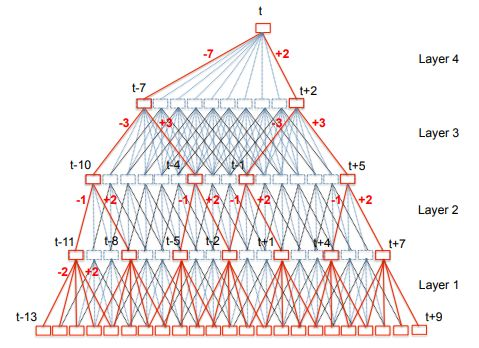
\includegraphics[scale=.62]{Images/tdnn.jpeg}}
\caption{ Computation in TDNN with sub-sampling (red) and
without sub-sampling (blue+red)~\cite{snyder2018spoken}.}
\label{tdnn}
\end{figure}

 \begin{table}
 \caption{The embedding DNN architecture~\cite{snyder2018spoken}.}
 \label{xvac_ar}
\centering\begin{tabular}{|c|c|c|c|}
\hline
Layer                                                   & Layer Context & Total Context & $Input \times Output$ \\ \hline
layer 1                                                 & {[}t-2,t+2{]} & 5             & $5F \times 512 $      \\ \hline
layer 2                                                 & \{t-2,t,t+2\} & 9             & $1536 \times 512$     \\ \hline
layer 3                                                 & \{t-3,t,t+3\} & 15            & $1536 \times 512$     \\ \hline
layer 4                                                 & \{t\}         & 15            & $512 \times 512$      \\ \hline
layer 5                                                 & \{t\}         & 15            & $512 \times 1500$     \\ \hline
\begin{tabular}[c]{@{}c@{}}Stats\\ Pooling\end{tabular} & {[}0,T)       & T             & $1500T \times 3000 $  \\ \hline
Segment 6                                               & \{0\}         & T             & $3000 \times 512 $    \\ \hline
Segment 7                                               & \{0\}         & T             & $512 \times 512$      \\ \hline
Softmax                                                 & \{0\}         & T             & $512 \times L $       \\ \hline
\end{tabular}
\end{table}

The architecture of the sub-sampling based TDNN is given in table~\ref{xvac_ar}. Suppose an input utterance have T feature vectors of F dimension. The input to the network is the concatenation of acoustic features of five frames (2 past, 2 future, 1 current), i.e. a $5*F$ dimension vector. The first five layers operate on speech frames with a small temporal context centered at the current frame t. The statistical pooling layer aggregates all T frame-level outputs from layer 5 and computes it mean and standard deviation (1500 dimension), then concatenate the mean and standard deviation to form 3000 dimension vector (for the whole utterance) and give input to the next layer. The output layer is a softmax layer having the language labels. From segment 6 or segment 7, the embedding vectors are extracted, and then, PLDA and cosine kernel scoring techniques are used to perform language recognition.   
% \section{Language identification, Language verification and Language diarization}
% Like speaker recognition, spoken language recognition can be also be viewed as:
% \begin{itemize}
%     \item Language identification
   
%     \item Language verification
%     \item Language diarization
% \end{itemize}
   
% 
% %\section{Background}
% \lettrine[lines=1]{\textbf{T}}{his} chapter outlines the ..... 
% 
% 
% \section{Section 1}
% "Section Description"
% 
% \section{Section 2}
% "Section Description" \cite{Cite01}, "Section Description"
% \begin{equation}
% \label{eq2}
% x = y + z
% \end{equation}
% 
% Equation \ref{eq1} adds 2 numbers.
% 
% 
% \section{Section 3}
% "Section Description"

\end{spacing} 